\section{Projektbeskrivelse}
\begin{wrapfigure}[50]{TR}{0.5\textwidth}
	\centering
		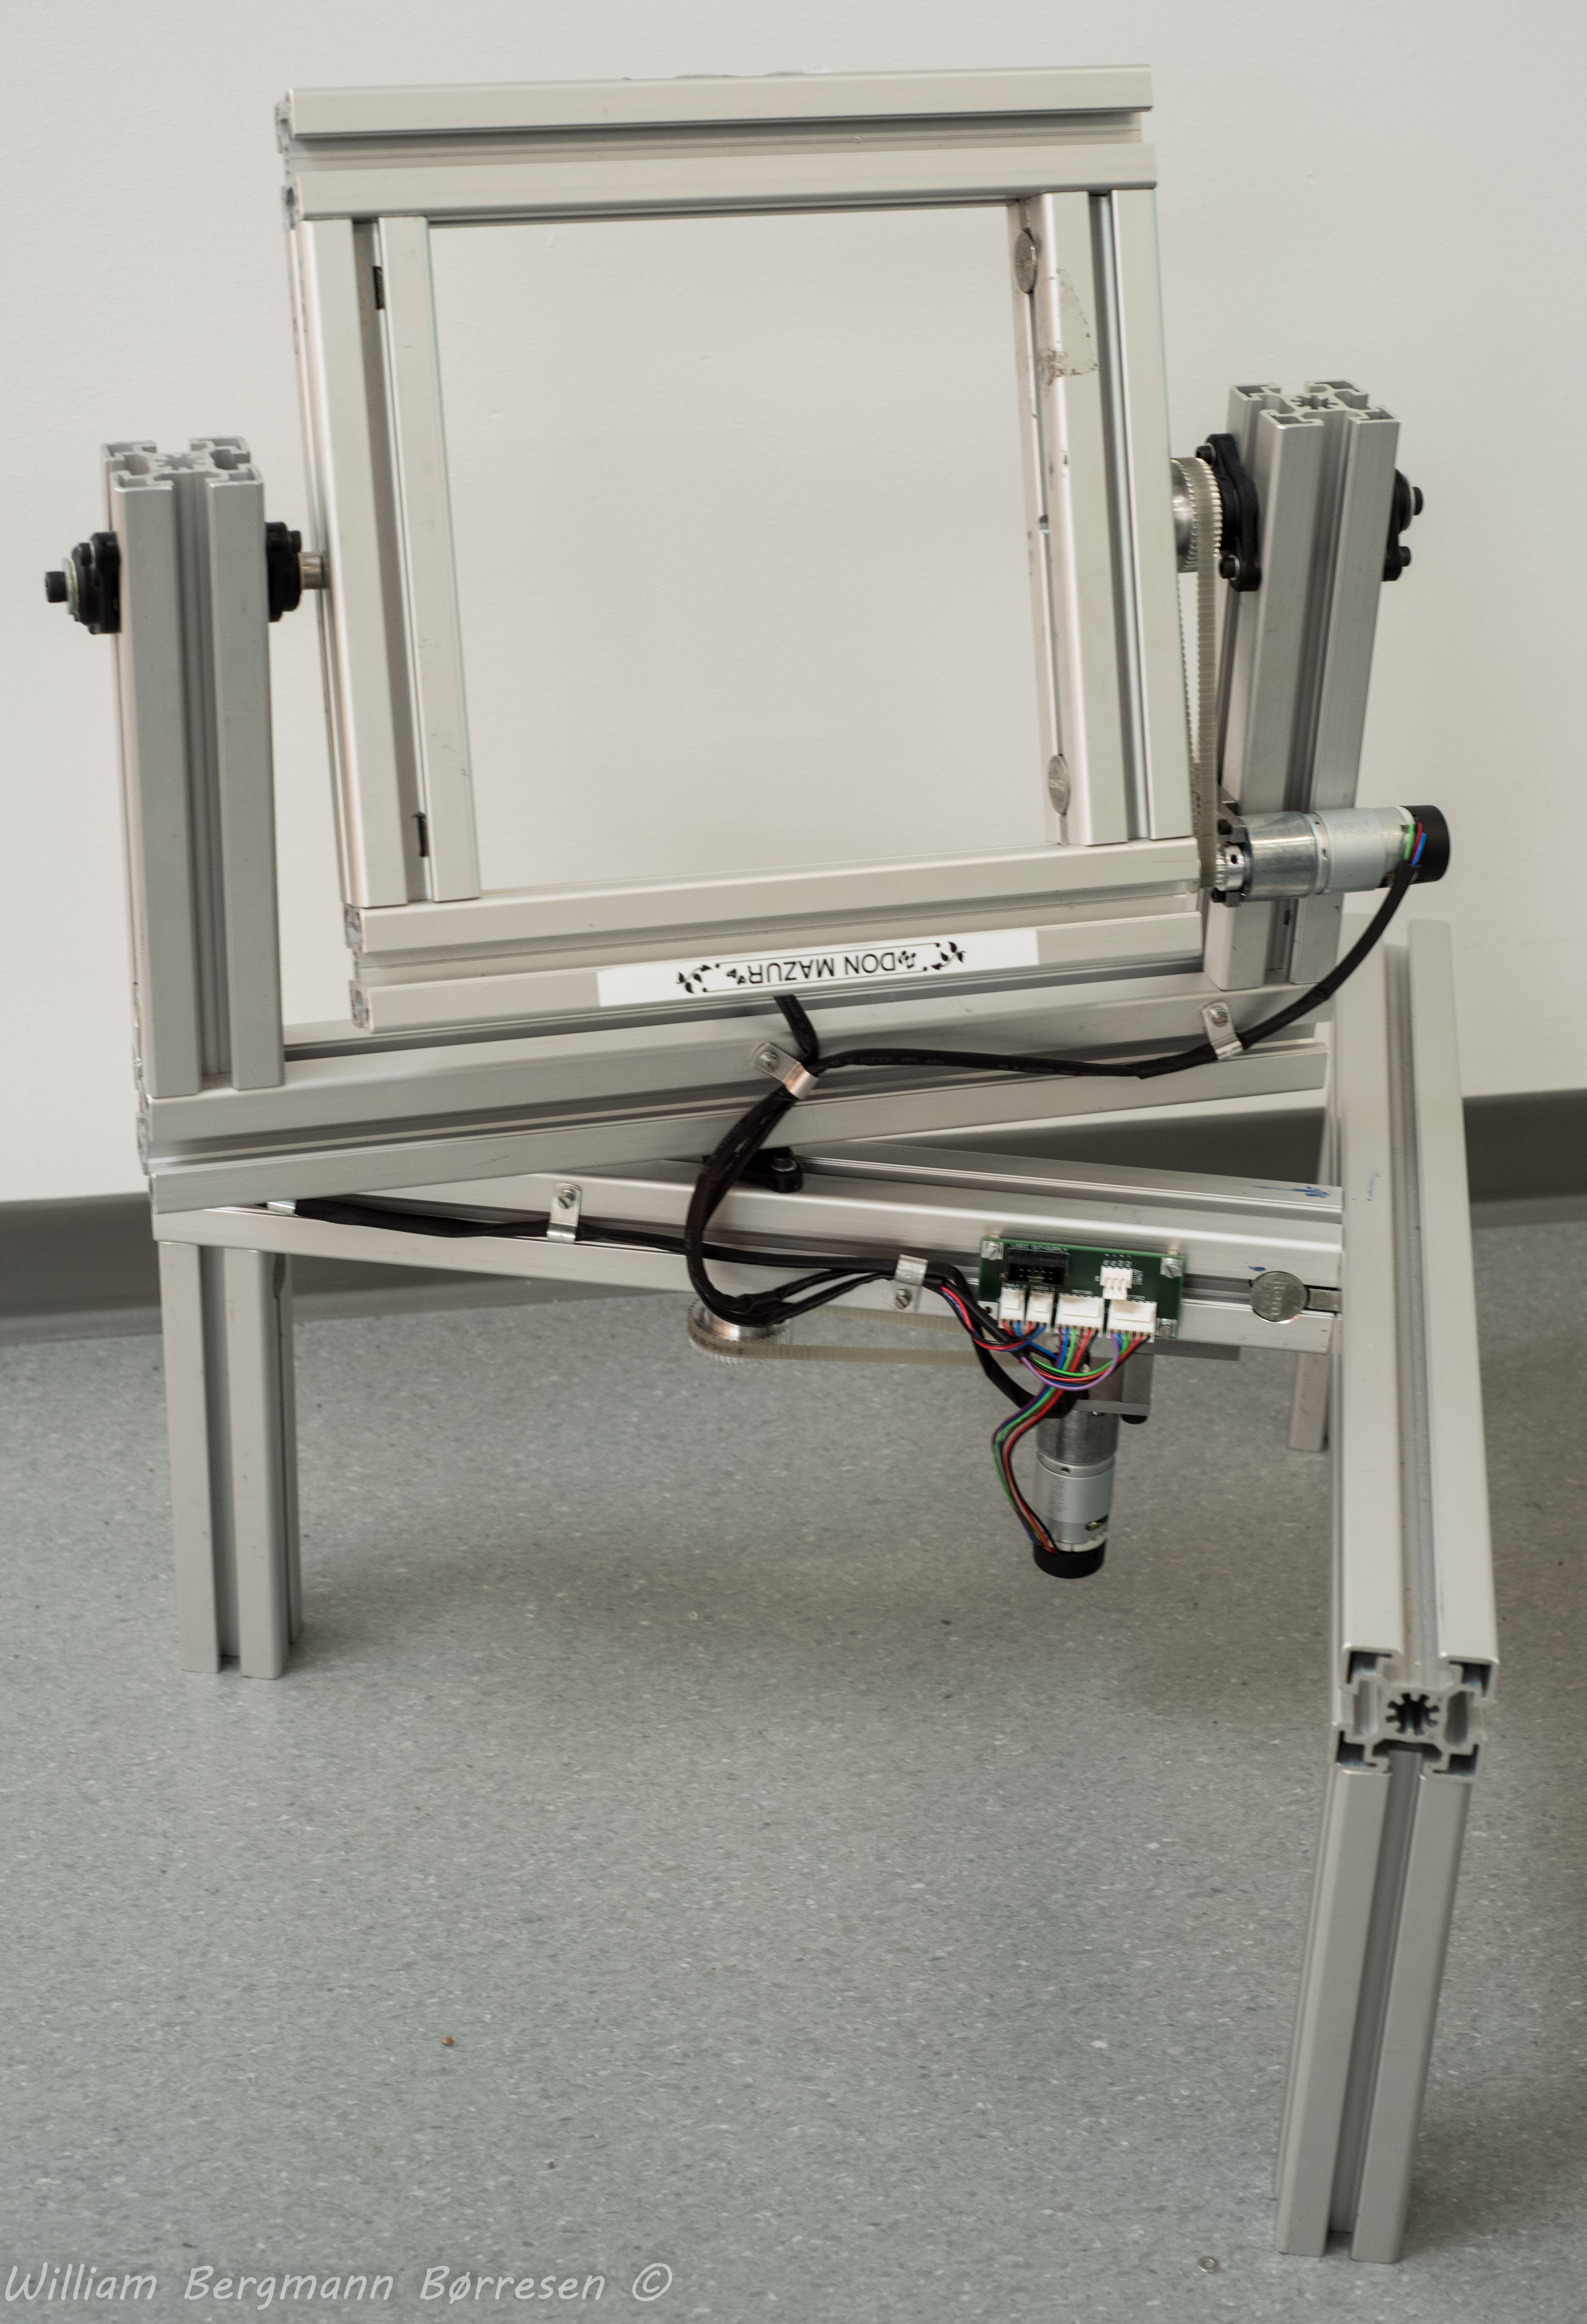
\includegraphics[scale=0.2]{Billeder/opstilling.jpg}
\caption{Opstilling af panorerings- og tilt-system med motorer og hall sensorer tilføjet.}
\label{fig:Opstilling}
\end{wrapfigure}
\subsection{Indledning}
Der er blevet tildelt et panorerings- og tilt-system, hvor tilt rammen er monteret på pan rammen.\\
Et sådan system bruges ofte til, observatorier, lysudstyr, overvågningskameraer iblandt mange andre applikationer.
Til følgende beskrivelse af systemet er der ønsket en valgfri meningsfyldt applikation, systemet kan ses på figur \ref{fig:Opstilling}.\\
For at pan rammen ikke river ledningerne i stykker til tilt rammen, er der tilføjet en stopklods, derfor har pan rammen en begrænsning, hvor tilt rammen er ubegrænset i dens bevægelser.\\
til rammerne er der tilføjet to EMG30\cite{emg30Data}, en på hhv pan og tilt rammerne.\\
På rammerne er også tilføjet 2 hall sensorer, en på pan, og en på tilt. 








%Dette projekt vil fokusere på at følge himmellegemer med en platform magen til et observatorium. Dette bliver implementeret ved at give systemet et horisontalt koordinatsæt, enten udregnet via en computer, eller via et numerisk tastatur som er blevet udleveret.\\
%Ved input fra en computer, vil der være mulighed for at lave en applikation, der automatisk følger et himmellegeme, ved at ændre koordinatsættet kontinuert.
%Systemet vil vise data på et LCD som er blevet udleveret, her vil det være muligt at observere hvilke nuværende koordinatsæt systemet har.\\
%XXXX Eventuelt nævne menu systemet herunder.\\

\subsection{Problemformulering}
Med dette project håber vi at finde ud af nyttige metoder til at styre et pan og tilt system ved brug af polære koordinater, som er nyttige i denne sammenhæng fordi der er nemme at omregne til og fra i forhold til andre koordinat systemer, samt meget intuitiv at benytte til et drejende system. Til dette er vi givet et pan og tilt system der har visse begrænsninger i dens mekaniske bevægelser. Vi skal derfor også finde en metode til at sikre at der ikke sker mekaniske uheld ved at systemet går ud over sine grænser.
\\
Når disse er opfyldt skal det undersøges om det er muligt at lave en matematisk model af systemet og dens opførsel, således at denne kan benyttes til at skabe et closed-loop kontrol system.\\

Efter at systemet er modeleret, skal der bygges en brugbar applikation til systemet, dette projekt vil derfor forsøge at implementere en platform hvorpå man kan montere et spejlrefleks kamera og tage billeder af himmellegemer.\\
Dette projekt vil derfor fokusere høj nøjagtighed.\\

\subsection{Kravspecifikation}

Hvis pan-tilt systemet skal pege på den internationale rumstation som bevæger sig i en afstand omkring 400 km væk fra jorden, og systemet er upræcist og bare peger en enkelt grad forkert, vil den næsten pege 7 km ved siden af.

\subsubsection{Arbejds- og fagområder}
Pan-Tilt projektet bliver udarbejdet for at give en bredere og bedre forståelse for det 4. semesters fag, derfor er der valgt nogle arbejds- og fag- områder som sørger for at projektet kommer til at have indhold fra hvert fag.\\
4. semester fagene består af:
\begin{itemize}[noitemsep]
	\item Computer Operativ Systemer (COS)
	\item Embedded Programmering (EMP)
	\item Reguleringsteknik (REG)
	\item Digital Programmerbar Elektronik (DIG)
\end{itemize}

\subsubsection{Obligatoriske Krav}

\begin{itemize}[noitemsep]
	\item COS/EMP
	\begin{itemize}[noitemsep]
		\item Task-baseret OS med schedulering
		\item SPI-Kommunikation mellem microcontroller og FPGA
	\end{itemize}
	\item REG
	\begin{itemize}[noitemsep]
		\item System analyse og modellering af systemets enkelte elementer
		\item Closed-loop controller
	\end{itemize}
	\item DIG
	\begin{itemize}[noitemsep]
		\item SPI-protokol til FPGA
		\item PWM driver til FPGA
		\item Motor position skal bestemmes af FPGA
	\end{itemize}
\end{itemize}

\subsubsection{Primære opgaver}

Som krav til systemet skal det kunne tage et input i form af et horizontalt koordinatsæt, som systemet så omsætter til angulære koordinater således dette kan benyttes af systemet. Yderligere er det nødvendigt at systemet kan tage manuelt indtastning af koordinater som alternativt input.

Som en del af COS/EMP faget sættes der som krav at systemet skal kunne give feedback gennem LCD komponenten i form af den nuværende position i astronomiske koordinater. Der skal kunne tages input fra knapper på EMP bordet, og en UART forbindelse, med tilsvarende UART protokol, skal kunne forbinde boardet med en computer.

Der skal laves en PID controler, som beskrevet i REG, som er foruden både overshoot og steady state fejl. Yderligere skal denne kunne bevæge sig 180 grader og stoppe på under fem sekunder, med en usikkerhed på højst én grad.

Samtidig skal der laves et stykke funktionelt digitalt programmeret elektronik, i form af et FPGA board, der skal fungerer som en ``slave'' for microcontrolleren og give denne information om positionen af systemet samt benytte denne til at sætte hastighed or retning på motorerne. Denne skal også fungerer som en sikkerhed der endegyldigt sikre at der ikke kan ske uheld ved at systemet kører ud over sine mekaniske begrændsninger.

\subsubsection{Sekundære opgaver}

De sekundære krav til systemet som helhed, og tilsvarende applikation, er at dette kan udregne baner for himmellegemer og hente live oplysninger fra internettet om legemers position. Yderligere skal systemet kunne styres ved brug af en direkte kontrol af position uden brug af koordinater, og et kamera skal monteres i pan tilt systemet. Endeligt skal et bluetooth modul kunne benyttes til UART kommunikation.

Til COS/EMP fagene er det sekundære krav at systemet kan overvåges gennem UART, således at der kan holdes styr på performance af kontroleren og hvorvidt den ønskede position er overholdt, således at der kan tages automatiske billeder.

Det sekundære krav til REG er at PID controlleren er i stand til at selvkalibrerer til et givent system.

Til DIG er det sekundære krav at denne er i stand til at omregne til omregne systemets koordinater til grader.